%for impressive
\pdfminorversion=4

\documentclass{beamer}
\usetheme{Warsaw}
\setbeamertemplate{navigation symbols}{}

\usepackage{xcolor,colortbl}
\usepackage{tikz}
\usepackage{graphicx}
\usepackage{hyperref}

%pl lang
\usepackage{polski}
\usepackage[utf8]{inputenc}
\usepackage[polish]{babel}

\useoutertheme{shadow}
\useinnertheme[shadow=true]{rounded}

%fixing headers and footers :P
\setbeamertemplate{headline}{}
\setbeamercolor{mycolor}{fg=white,bg=black}

\defbeamertemplate*{footline}{shadow theme}{%
\leavevmode%
\hbox{\begin{beamercolorbox}[wd=.1\paperwidth,ht=2.5ex,dp=1.125ex,leftskip=.3cm plus1fil,rightskip=.3cm]{author in head/foot}%
    \usebeamerfont{author in head/foot}\hfill\insertshortauthor
\end{beamercolorbox}%
\begin{beamercolorbox}[wd=.8\paperwidth,ht=2.5ex,dp=1.125ex,leftskip=.3cm,rightskip=.3cm plus1fil]{title in head/foot}%
    \usebeamerfont{title in head/foot}\insertshorttitle\hfill%
\end{beamercolorbox}%
\begin{beamercolorbox}[wd=.1\paperwidth,ht=2.5ex,dp=1.125ex,leftskip=.3cm,rightskip=.3cm plus1fil]{mycolor}%
\hfill\insertframenumber\,/\,\inserttotalframenumber
\end{beamercolorbox}}%
\vskip0pt%
} 

        
\title{Introduction to GIT}
\date{June 2014}


\begin{document}



%  ---   Begin ---


		
	\section{Welcome}
		\subsection{Hi mum!}
		\begin{frame}
			\frametitle{Hi mum!}
			\begin{center}
				
\includegraphics[scale=0.7]{images/gitmeme}
			\end{center}
		\end{frame}
		

%  ---   Why git ---

	\section{Why git?}
		\subsection{Killer feature}
		\begin{frame}
			\frametitle{Killer feature: Cheap Local Branching}
			\begin{center}
				
\includegraphics[scale=1]{images/fact1}
			\end{center}
		\end{frame}


    \subsection{Workflow}
		\begin{frame}
			\frametitle{Supports any Workflow, Subversion-Style}
			\begin{center}
				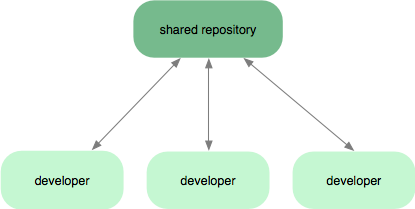
\includegraphics[scale=1]{images/fact4_1}
			\end{center}
		\end{frame}	

		\begin{frame}
			\frametitle{Supports any Workflow, Integration Manager}
			\begin{center}
				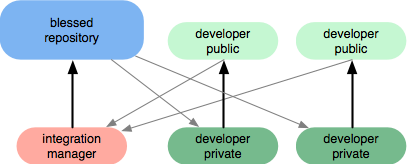
\includegraphics[scale=1]{images/fact4_2}
			\end{center}
		\end{frame}	
		
		\begin{frame}
			\frametitle{Supports any Workflow, Dictator and Lieutenants}
			\begin{center}
				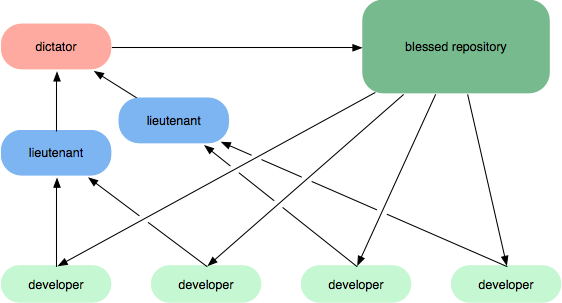
\includegraphics[scale=1]{images/fact4_3}
			\end{center}
		\end{frame}	

		\begin{frame}
			\frametitle{Pro: fast}
			\begin{center}
				\begin{tabular}{ l  c  c  c }
				    \hline
						& Git & Hg & Bzr \\ \hline
						Init & \cellcolor{green!25} 0.024s & 0.059s & 0.600s \\ \hline
						Add & 8.535s & \cellcolor{green!25} 0.368s & 2.381s \\ \hline
						Status & \cellcolor{green!25} 0.451s & 1.946s & 14.744s \\ \hline
						Diff & \cellcolor{green!25} 0.543s & 2.189s & 14.248s \\ \hline
						Tag & \cellcolor{green!25} 0.056s & 1.201s & 1.892s \\ \hline
						Log & \cellcolor{green!25} 0.711s & 2.650s & 9.055s \\ \hline
						Commit (Large) & \cellcolor{green!25} 12.480s & 12.500s & 23.002s \\ \hline
						Commit (Small) & \cellcolor{green!25} 0.086s & 0.517s & 1.139s \\ \hline
						Branch (Cold) & \cellcolor{green!25} 1.161s & 94.681s & 82.249s \\ \hline
						Branch (Hot) & \cellcolor{green!25} 0.070s & 12.300s & 39.411s \\ \hline
				\end{tabular}
				\\ 
				1) "The following are a number of benchmarks that I performed on three copies of the Django source code repository" \\
				2) add operation over 2000 files
			\end{center}
		\end{frame}
		
		\begin{frame}
			\frametitle{Pro: fast 2}
			\begin{center}
				\small
				\begin{tabular}{ l  c  c  c c }
				    \hline
				     Info & Git  & SVN & Magn. \\ \hline
\tiny Commit Files (A) - Add, commit and push 113 modified files (2164+, 2259-) &  0.64 &  2.60 & 4x \\ \hline
\tiny Commit Images (B) - Add, commit and push 1000 1k images &  1.53 & 24.70 & 16x \\ \hline
\tiny Diff Current - Diff 187 changed files (1664+, 4859-) against last commit &  0.25 &  1.09 & 4x \\ \hline
\tiny Diff Recent - Diff against 4 commits back (269 changed/3609+,6898-) &  0.25 &  3.99 & 16x \\ \hline
\tiny Diff Tags - Diff two tags against each other (v1.9.1.0/v1.9.3.0 ) &  1.17 & 83.57 & 71x \\ \hline
\tiny Log (50) - Log of the last 50 commits (19k of output) &  0.01 &  0.38 & 31x \\ \hline
\tiny Log (All) - Log of all commits (26,056 commits - 9.4M of output) &  0.52 & 169.20 & 325x \\ \hline
\tiny Log (File) - Log of the history of a single file (array.c - 483 revs) &  0.60 & 82.84 & 138x \\ \hline
\tiny Update - Pull of Commit A scenario (113 files changed, 2164+, 2259-) &  0.90 &  2.82 & 3x \\ \hline
\tiny Blame - Line annotation of a single file (array.c) &  1.91 &  3.04 & 1x \\ \hline
				\end{tabular}
			\end{center}
		\end{frame}				

		\begin{frame}
			\frametitle{Pros}
			\begin{center}
				%\makebox[\textwidth]{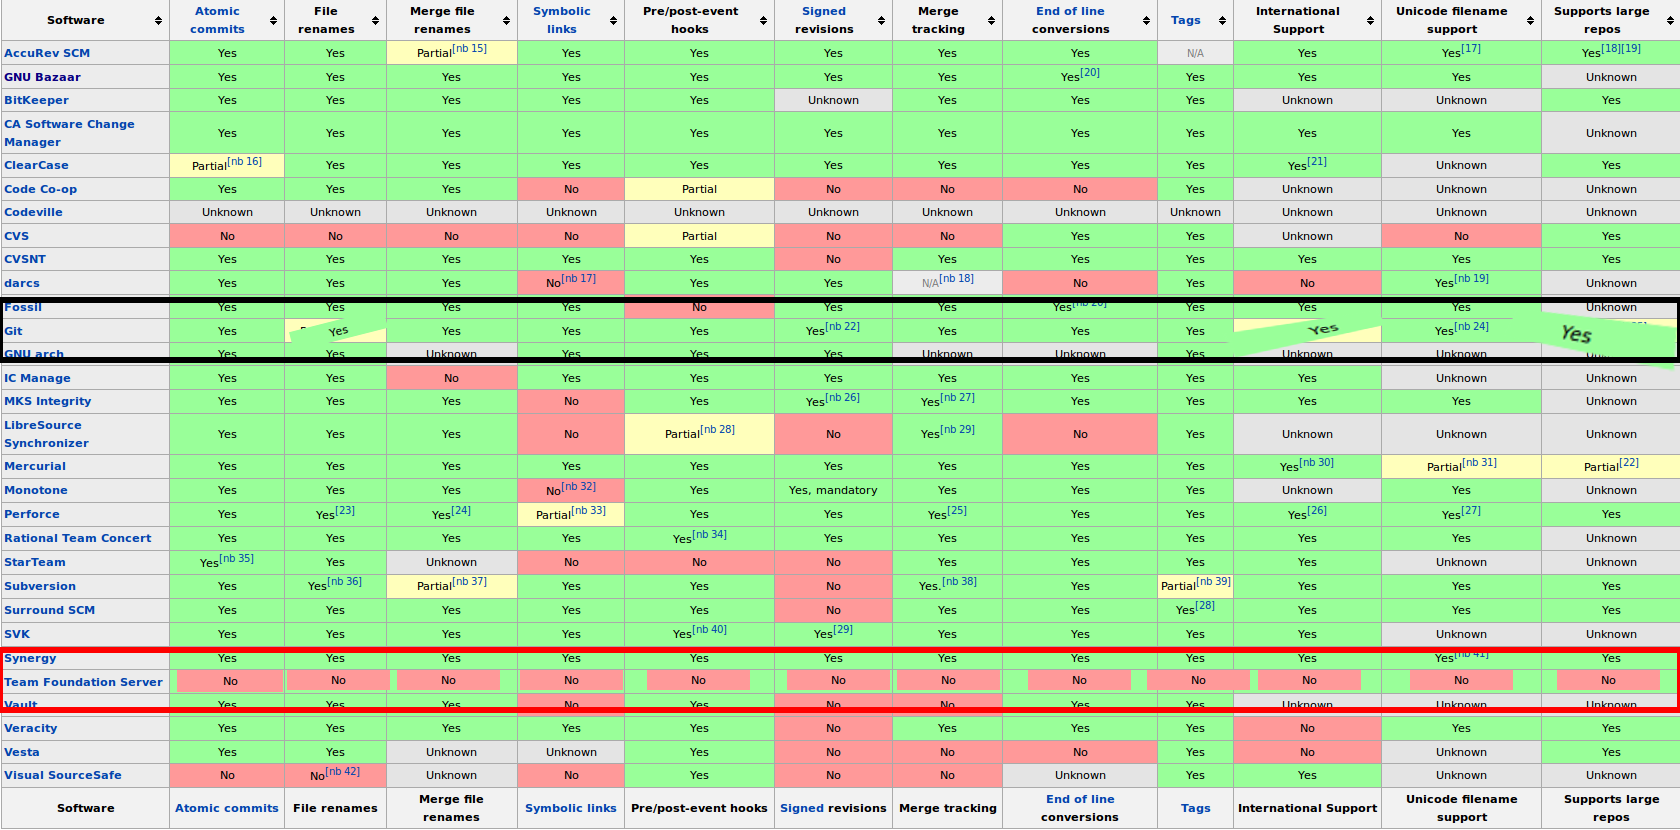
\includegraphics[width=\paperwidth]{images/why}}
			\begin{itemize}
                \item Designed for distributed, non-linear, large-scale projects
                \item Makes 'take a small step' development very simple
                \item Improves clear communication about changes 
                \item Encourages experimenting and contributing
                \item Implicit backup
                \item see: \href{https://github.com/git/git/commit/1ca41a19323d455cf0028001677f3adfae0d4cc4}{perfect commit in git}
			\end{itemize}
			\end{center}
		\end{frame}

		\subsection{Standard}

		\begin{frame}
			\frametitle{Pro: de facto standard 1}
      the most widely adopted version control system for software development
			\begin{columns}
				\column{.3\textwidth}
					\begin{itemize}
					\item Linux Kernel
					\item OpenVZ
					\item KVM
					\item Android
					\item Bacula
					\item dash
					\item Drupal
					\item FFmpeg
					\item GCC
					\item GNOME
					\item jQuery
					\end{itemize}
				\column{.3\textwidth}
					\begin{itemize}
					\item Mantis
					\item Openbox
					\item Perl5
					\item PulseAudio
					\item Puppet
					\item Qt
					\item Ruby on Rails
					\item VLC
					\item Wine
					\item x264
					\item YUI3
					\end{itemize}
				\column{.3\textwidth}
					\begin{itemize}
					\item Google
					\item facebook
					\item Microsoft
					\item twitter
					\item LinkedIn
					\item Netflix
					\item Apache Camel
					\item Eclipse
					\item PostgreSQL
					\item X
					\item KDE
					\end{itemize}
			\end{columns}
		\end{frame}	

		\begin{frame}
			\frametitle{Pro: de facto standard 2}
			\begin{center}
				\makebox[\textwidth]{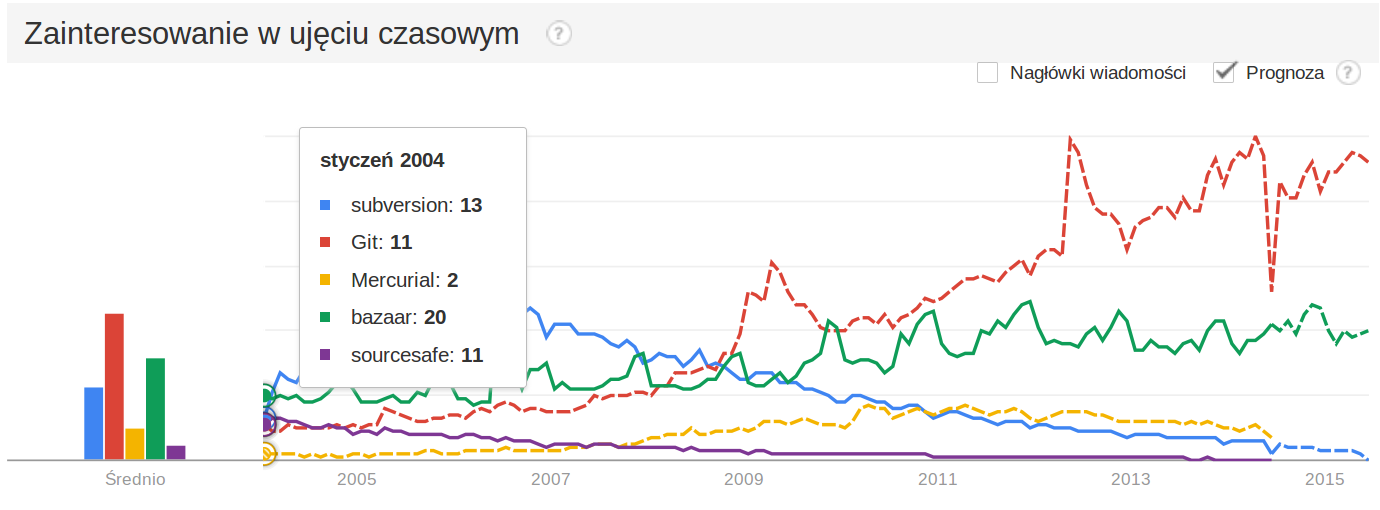
\includegraphics[width=\paperwidth]{images/why2}}
			\end{center}
		\end{frame}
		
		\begin{frame}
			\frametitle{Pro: de facto standard 3}
			\begin{center}
				\makebox[\textwidth]{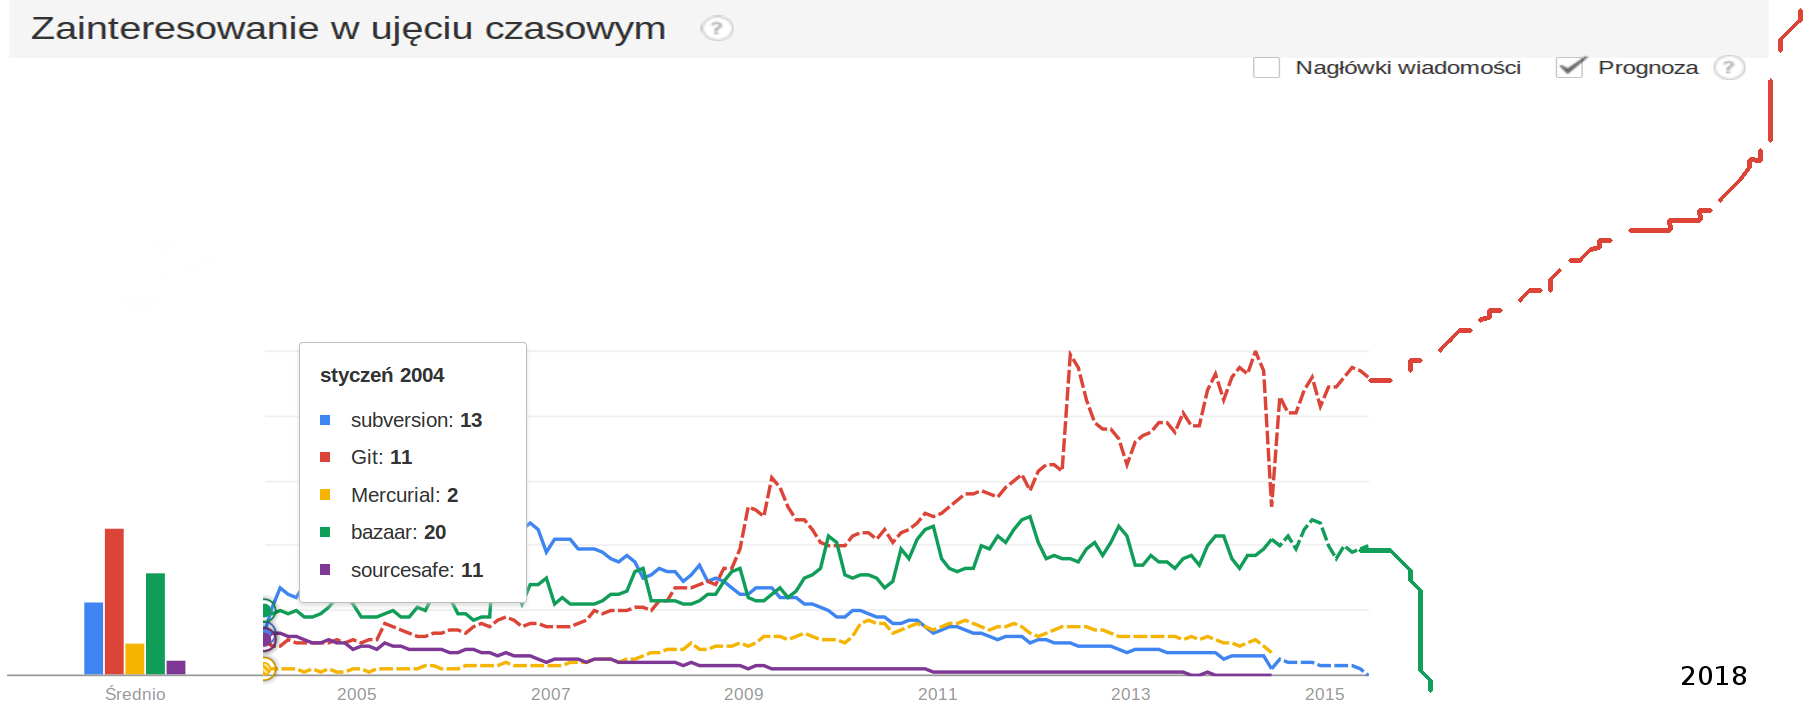
\includegraphics[width=\paperwidth]{images/why3}}
			\end{center}
		\end{frame}


    \subsection{Cons}
		\begin{frame}
			\frametitle{Cons}
			\begin{center}
				%\makebox[\textwidth]{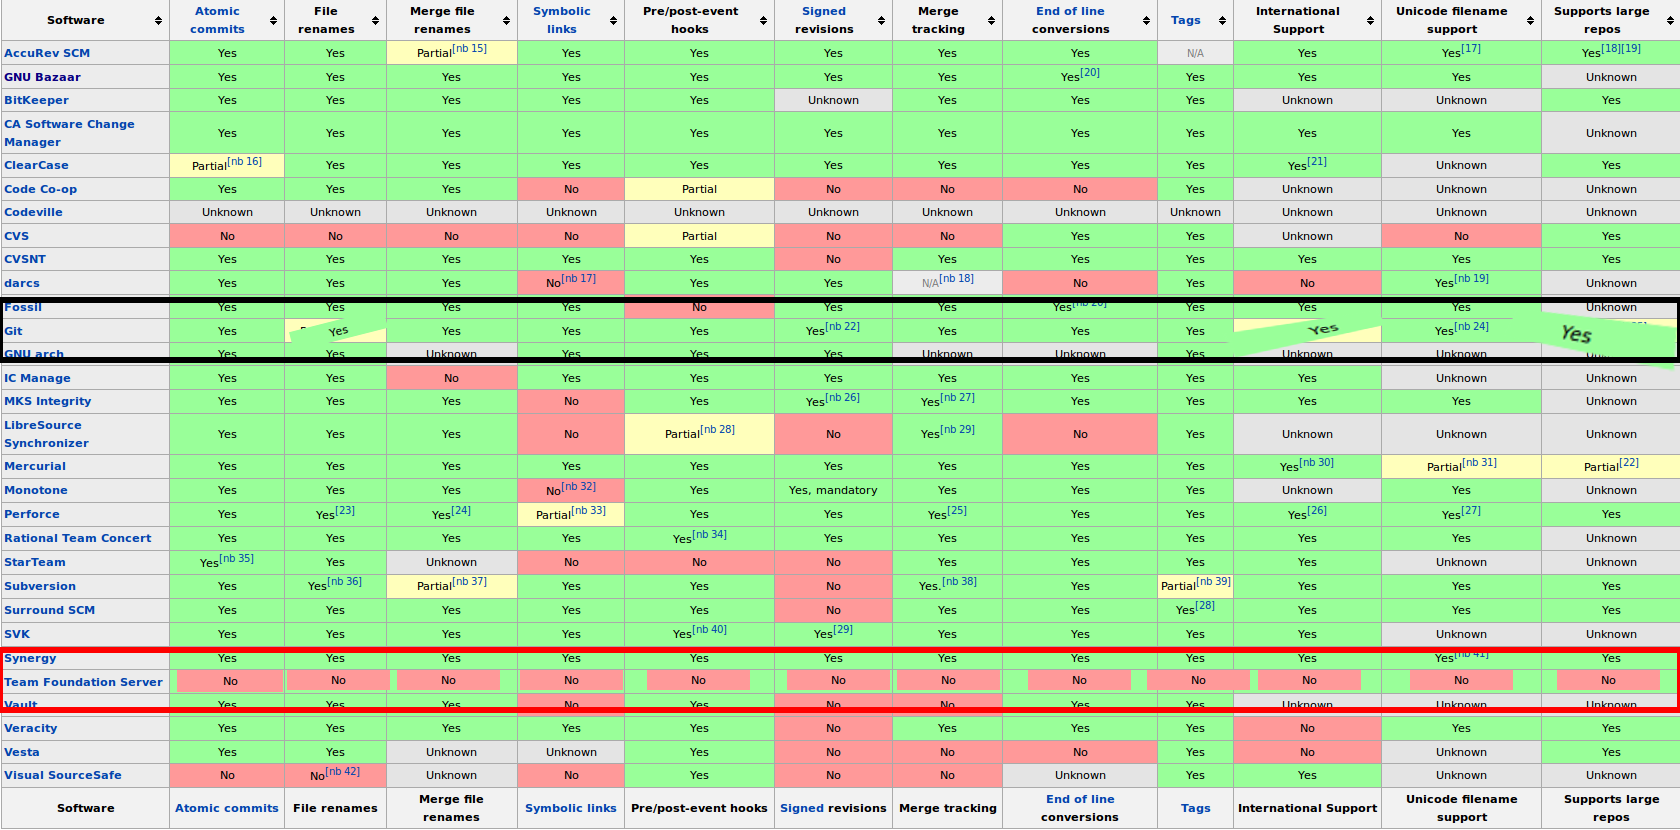
\includegraphics[width=\paperwidth]{images/why}}
			\begin{itemize}

        \item Complex, 'controlling complexity is the essence of computer programming', Brian Kernighan
        \item Powerful, 'with great power comes great responsibility', Voltaire
        \item Cryptic command-line vocabulary
        \item Puts off integration
			\end{itemize}
			\end{center}
		\end{frame}

    \subsection{SVN pros}
		\begin{frame}
			\frametitle{Contrast: SVN Pros}
			\begin{center}
			\begin{itemize}
        \item Everybody knows it
        \item Simple
        \item Code integration happens quickly and often
			\end{itemize}
			\end{center}
		\end{frame}	

%  ---   Commit stages ---

	\section{Stages}
		\subsection{Overview}
		\begin{frame}
			\frametitle{Commit stages: overview}
			\begin{center}
				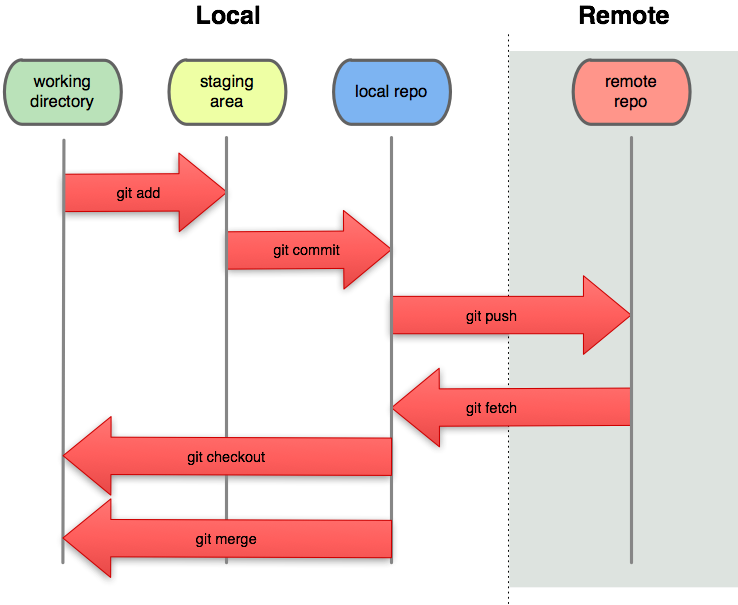
\includegraphics[scale=0.8]{images/fact2}
			\end{center}
		\end{frame}

		\subsection{Details}
		\begin{frame}
      \frametitle{Commit stages: basic actions}
			\begin{center}
			\begin{itemize}
        \item Commit represents changeset identified by hash
        \item Commit stages:
			  \begin{itemize}
            \item Untracked, not staged, working directory 
            \item Staging area, index 
            \item Repository, committed changes
        \end{itemize}
        \item Remove from staging area: git reset
        \item Change/select commit to start working off: git checkout
			\end{itemize}
			\end{center}
		\end{frame}

		\begin{frame}
      \frametitle{Commit stages: checking status}
			\begin{center}
			\begin{itemize}
        \item git status
        \item untracked vs. staging: git diff
        \item staging vs. repository: git diff -{}-cached
			\end{itemize}
			\end{center}
		\end{frame}

		\subsubsection{DAG: Version graph}
		\begin{frame}
			\frametitle{DAG: Version graph}
			\begin{center}
				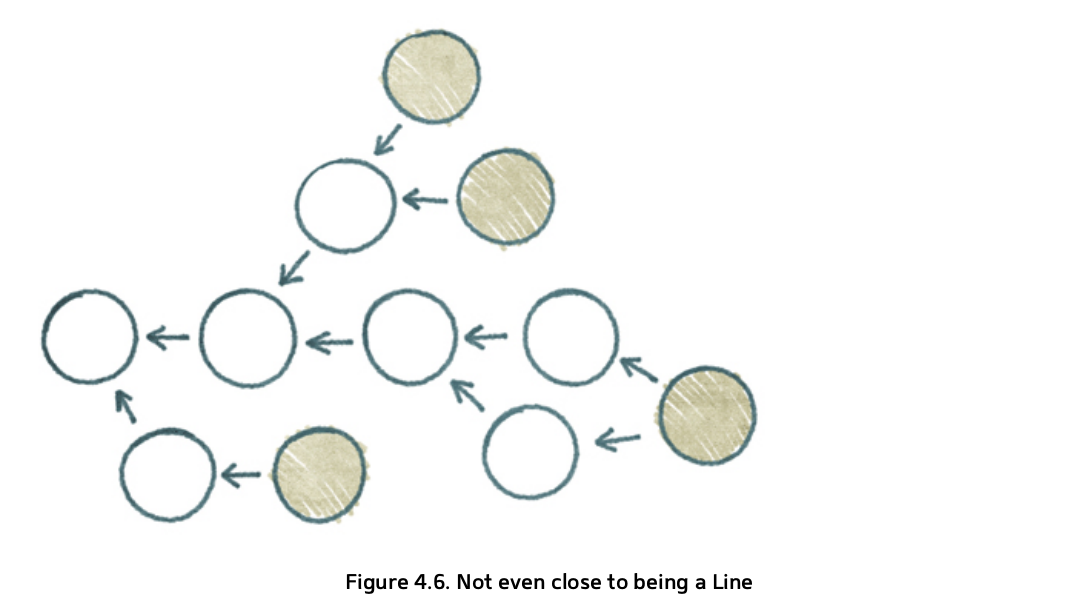
\includegraphics[scale=0.3]{images/dag}
			\end{center}
		\end{frame}

		\begin{frame}
			\frametitle{DAG: Version graph 2}
			\begin{itemize}
        \item Node is a changeset
        \item Directed edge means "is based on"
        \item Branch is a pointer, master is a special branch
        \item HEAD is a pointer to branch pointer
        \item HEAD gives a view of the current version
        \item Detached HEAD means HEAD points directly at a node
        \item Commit with 2+ parents is a result of (non-ff) merge
        \item git log -{}-graph: shows version graph
			\end{itemize}
			\begin{center}
			\end{center}
		\end{frame}

%  ---   Commands ---
		
		\subsubsection{git Commands}
		\begin{frame}
			\frametitle{git commands}
			\begin{center}
				
\includegraphics[scale=.5]{images/commands}
			\end{center}
		\end{frame}

		\subsubsection{init}
		\begin{frame}
			\frametitle{init}
			\begin{columns}
				\column{.4\textwidth}
				git init . \\
				git init -{}-bare .\\

				\column{.5\textwidth}
			\end{columns}
		\end{frame}

		\subsubsection{clone}
		\begin{frame}
			\frametitle{clone}
			\begin{columns}
				\column{.4\textwidth}
				git clone URL

				\column{.5\textwidth}
			\end{columns}
		\end{frame}

		\begin{frame}
			\frametitle{clone 2}
			\begin{itemize}
				\item ssh://[user@]host.xz[:port]/path/to/repo.git/
					\begin{itemize}
						\begin{columns}
							\column{.3\textwidth}
							easy to set up, authenticated

							\column{.3\textwidth}
							no anonymous access
						\end{columns}
					\end{itemize}
				\item git://host.xz[:port]/path/to/repo.git/
					\begin{itemize}
						\begin{columns}
							\column{.3\textwidth}
							fastest

							\column{.3\textwidth}
							lack of authentication
						\end{columns}
					\end{itemize}
				\item http[s]://host.xz[:port]/path/to/repo.git/
					\begin{itemize}
						\begin{columns}
							\column{.3\textwidth}
							easy to set up

							\column{.3\textwidth}
							inefficient, lot more network overhead
						\end{columns}
					\end{itemize}
				\item ftp[s]://host.xz[:port]/path/to/repo.git/
				\item rsync://host.xz/path/to/repo.git/
			\end{itemize}
			\begin{itemize}
				\item ssh://[user@]host.xz[:port]/~[user]/path/to/repo.git/
				\item git://host.xz[:port]/~[user]/path/to/repo.git/
				\item {[user@]}host.xz:/~[user]/path/to/repo.git/
			\end{itemize}
			\begin{itemize}
				\item /path/to/repo.git/
				\item file:///path/to/repo.git/
			\end{itemize}
		\end{frame}

		\subsubsection{push}
		\begin{frame}
			\frametitle{push}
			\begin{columns}
				\column{.4\textwidth}
				git push\\
				git push repository\\
				git push repository refspec\\
				\begin{center}
					
\includegraphics[scale=.2]{images/git_starwars}
				\end{center}

				\column{.5\textwidth}
			\end{columns}
		\end{frame}


		\subsubsection{merge fast-forward}
		\begin{frame}
			\frametitle{merge fast-forward 1}
        Having this: \\
				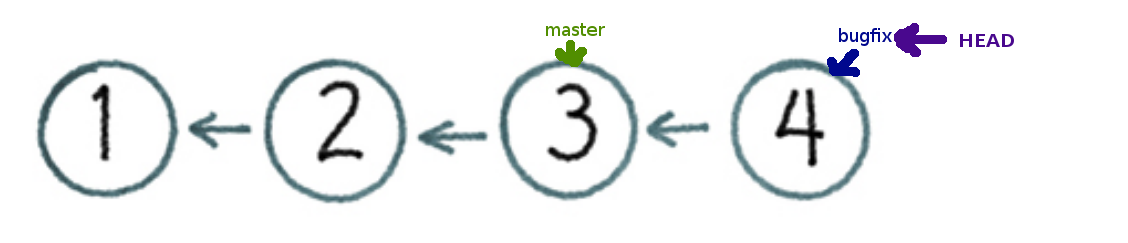
\includegraphics[scale=0.3]{images/merge_ff1}\\
        Let us merge: \\
        git checkout master \\
        git merge -{}-ff bugfix \\
		\end{frame}

		\begin{frame}
			\frametitle{merge fast-forward 2}
        Result: \\
				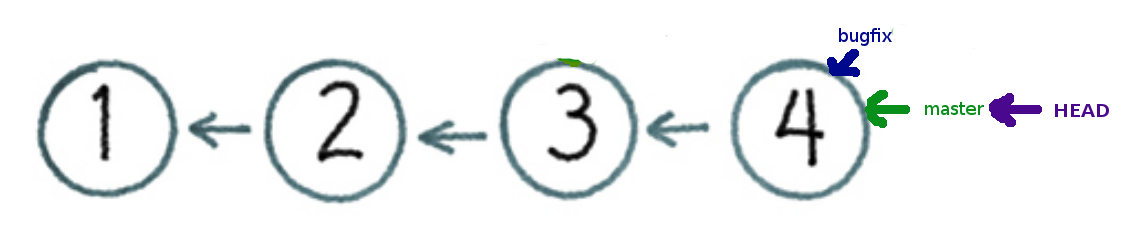
\includegraphics[scale=0.3]{images/merge_ff2}
		\end{frame}

		\subsubsection{merge no-fast-forward}
		\begin{frame}
			\frametitle{merge no-fast-forward 1}
        Having this: \\
				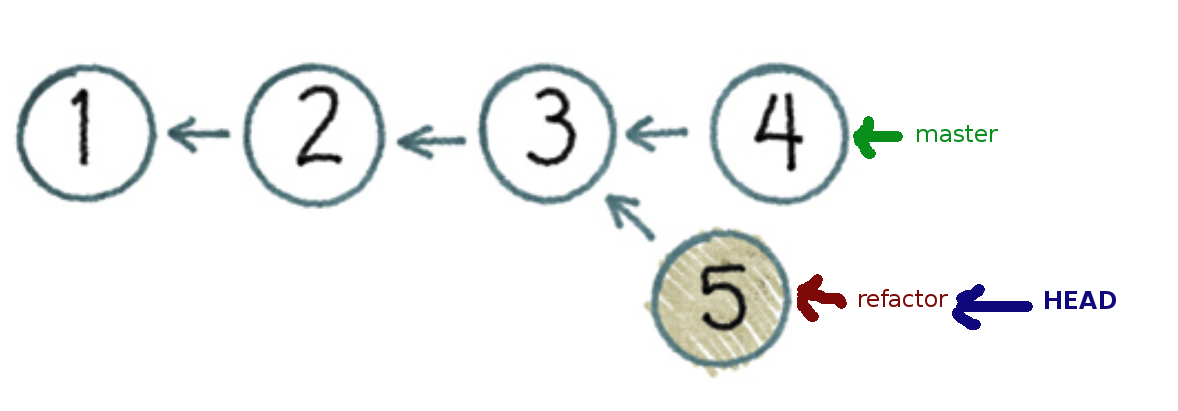
\includegraphics[scale=0.25]{images/merge_noff1}\\
        Let us merge without fast-forward: \\
        git checkout master \\
        git merge -{}-no-ff refactor \\
		\end{frame}

		\begin{frame}
			\frametitle{merge no-fast-forward 2}
        Result: \\
				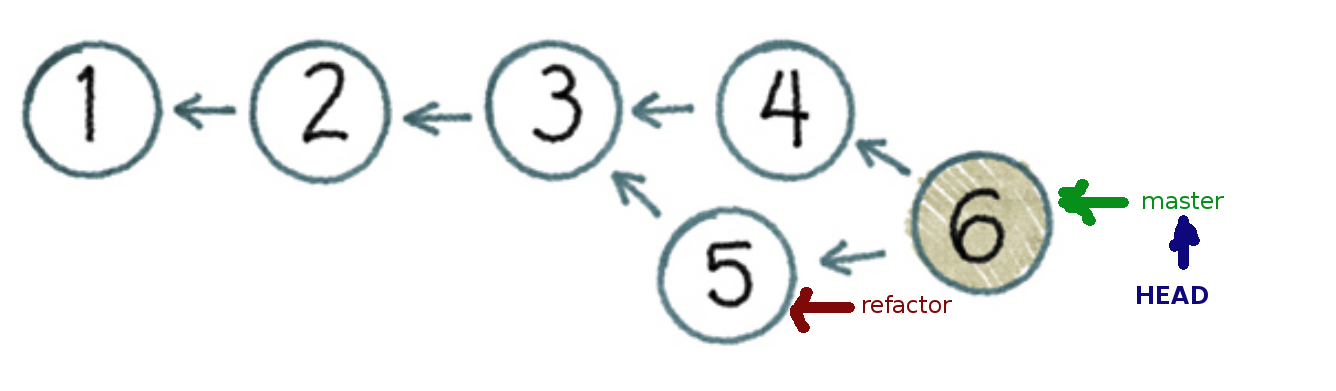
\includegraphics[scale=0.25]{images/merge_noff2}
		\end{frame}

		\subsubsection{rebase}
		\begin{frame}
			\frametitle{git rebase 1}
        Having this: \\
				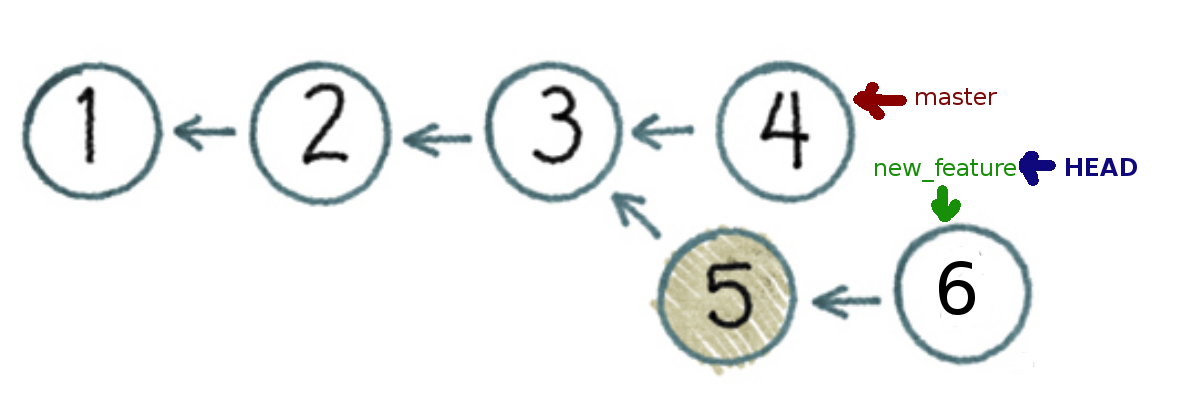
\includegraphics[scale=0.25]{images/rebase1} \\
        Let us rebase: \\
        git checkout new\textunderscore feature \\
        git rebase master
		\end{frame}

		\begin{frame}
			\frametitle{rebase 2}
      Result: \\
				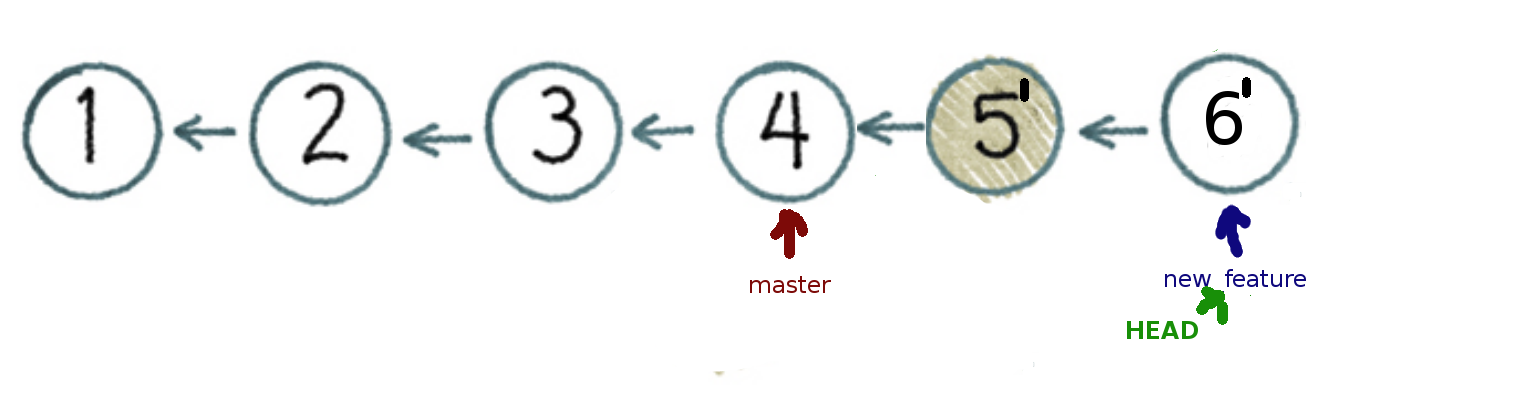
\includegraphics[scale=0.25]{images/rebase2}
		\end{frame}

		\begin{frame}
			\frametitle{rebase 3}
				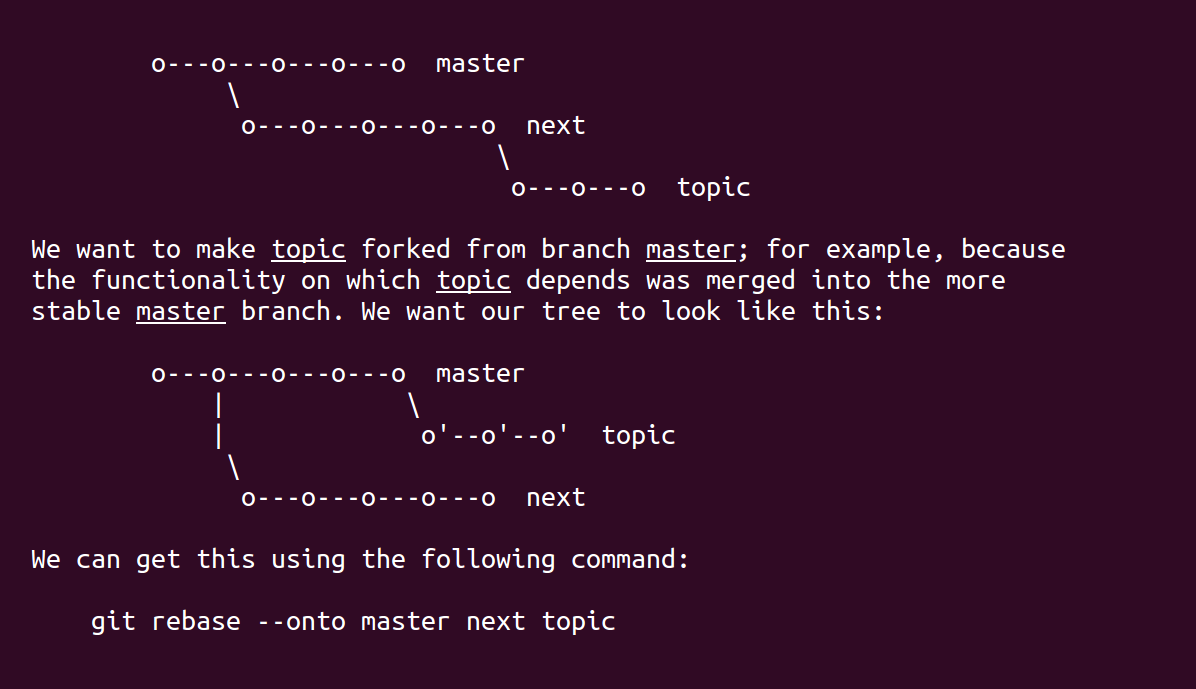
\includegraphics[scale=0.25]{images/rebase-into}
		\end{frame}

		\begin{frame}
      \frametitle{rebase -{}-interactive}
			\begin{itemize}
          \item squash = combine commits
          \item reword = change commit message
          \item used to drop, reorder, split commits
          \item git rebase -i HEAD\textasciitilde 3 \# change last three commits
			\end{itemize}
		\end{frame}

		\begin{frame}
			\frametitle{cherry-pick}
			\begin{center}
				\makebox[\textwidth]{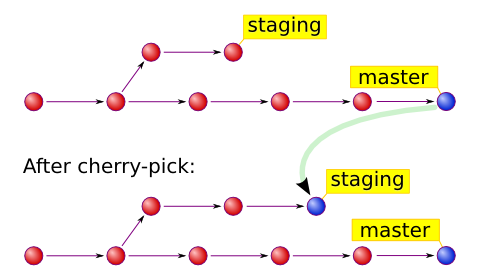
\includegraphics[scale=0.8]{images/git-cherry-pick}}
			\end{center}
			git checkout staging \: \: git cherry-pick master
		\end{frame}

		
%  ---   Branching and merging ---
		
	\section{Branching and merging}
				
		\subsection{Workshop}
		\begin{frame}
			\frametitle{Workshop}
		\end{frame}

%  ---   Najlepsze praktyki ---

	\section{Best practice}
		\subsection{Best practice}
		\begin{frame}
			\frametitle{Best practice}
			\begin{center}
				
\includegraphics[scale=2.5]{images/best-practice}
			\end{center}
		\end{frame}	
		
	\subsection{Best practice SM}
		\begin{frame}
			\frametitle{Best practice SM}
            Łukasz Rączka:
			\begin{itemize}
                \item binaries in git not recommended, repo slows down, hard to remove them
                \item git-svn: 4 attempts, not recommended, one person to merge repos (git and svn) through rebase
                \item separate repo per module, submodules: no good experience, semi-automatic solution
			\end{itemize}
		\end{frame}
		
	\subsection{Best practice SM \#2}
		\begin{frame}
			\frametitle{Best practice SM \#2}
            Marcin Książek:
			\begin{itemize}
                \item use git central repo, add prefix for your repo to group all project repos
                \item biggest problem: people do not accept agreed rules, history re-write
                \item many smaller repos rather than one large
                \item SourceTree recommended (better version on Mac, no version on Linux)
                \item BeyondCompare - best but paid tool to merge (Lin/Win/Mac)
			\end{itemize}
		\end{frame}
				
	\subsection{Best practice: others}
		\begin{frame}
			\frametitle{Best practice: others}
			\begin{itemize}
                \item review changes before committing
                \item don't rewrite history
                \item small, logically concise commits:
			    \begin{itemize}
                    \item new feature
                    \item formatting
                    \item other feature
                    \item no-op refactoring
                    \item bug fix
                    \item new API
			    \end{itemize}
                \item commit early and often
			\end{itemize}
		\end{frame}
		
	\subsection{Best practice: others \#2}
		\begin{frame}
			\frametitle{Best practice: others \#2}
			\begin{itemize}
                \item commit message: explain your changes:
			    \begin{itemize}
                    \item first line: what? 
                    \item third line: how? why? problem description, changes in architecture, solution limitations
                \end{itemize}
                \item split work into repos
			    \begin{itemize}
                    \item conceptually
                    \item according to permisions
                    \item large binaries
                    \item repo for history re-write
                \end{itemize}
                \item don't panic, committed changes stay
                \item choose workflow
			\end{itemize}
		\end{frame}
		
		\begin{frame}
			\frametitle{Quiz}
			\begin{itemize}
                \item What are commit stages?
                \item What is commit?
                \item HEAD?
                \item Detached HEAD?
                \item Branch?
                \item DAG?
                \item Merge?
                \item Rebase?
                \item Rebase interactive?
                \item Cherry pick?
			\end{itemize}
		\end{frame}
		
%  ---   Thats all ---
		\begin{frame}
			\frametitle{That's not all.}
			\begin{itemize}
                \item Go through: LearnGitBranching
                \item Go through: GitHug
                \item Experiment on GitHub, GitLab, Stash
                \item Watch: Introduction to Git with Scott Chacon of GitHub
                \item Read free book: ProGit, Scott Chacon
                \item Find an expert
			\end{itemize}
		\end{frame}
		
\end{document}
